\documentclass[12pt,a4paper]{article}
\usepackage[english]{babel}
\usepackage[utf8]{inputenc}
\usepackage{amssymb,amsmath}
\usepackage[all]{xy}
\usepackage{url}
\usepackage{graphicx}
\usepackage{color}
\newcommand{\angstrom}{\textup{\AA}}
\color{black}
\usepackage{geometry}
\usepackage[autostyle]{csquotes}
\usepackage{tikz}
\usetikzlibrary{bayesnet}
\usepackage{dcolumn}
\usepackage{booktabs}
\usepackage{tikz}
\usetikzlibrary{positioning,shapes,arrows}
\newcolumntype{M}[1]{D{.}{.}{1.#1}}

\geometry{
	a4paper,
 	left=15mm,
 	right=15mm,
 	top=10mm,
 	bottom=15mm
}


\begin{document}
\title{Probabilistic Reasoning Homework}
\author{Michał Ostyk-Narbutt, 1854051}
\maketitle
\tableofcontents
\clearpage
\section{Bayes Networks}

\subsection{Variables}
CustodianWorking (C),  CustodianAsleep (CA), CustodianBusy (CB), AlarmWorking (W), Alarm (A), TopOfTheHour (T)
\subsection{Bayesian Network drawing}
\begin{figure}[h]
\centering


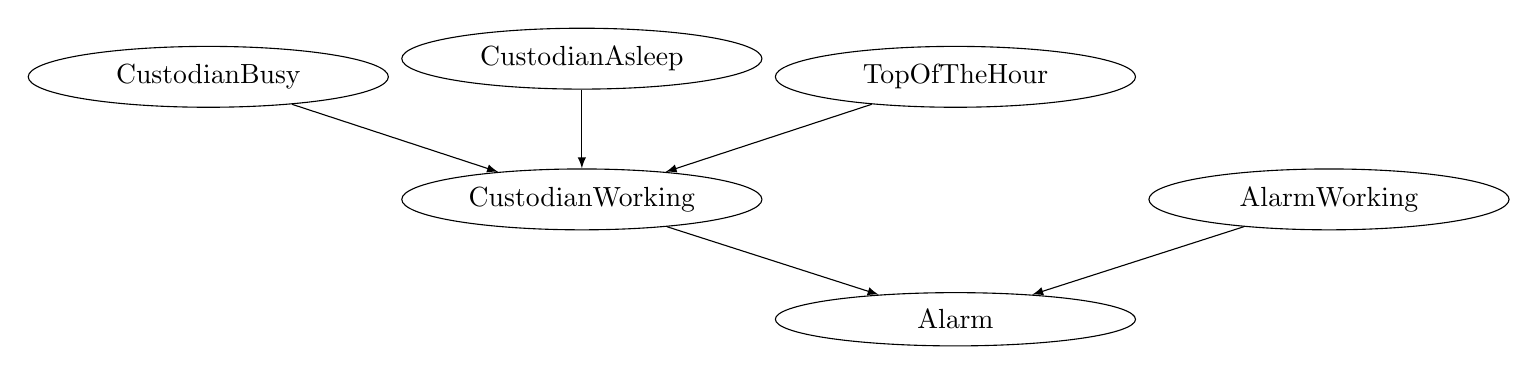
\begin{tikzpicture}[
  node distance=1cm and 1.5cm,
  mynode/.style={draw,ellipse,text width=3cm,align=center}
]
\node[mynode] (sp) {CustodianWorking};
\node[mynode, above right=of sp] (toth) {TopOfTheHour};
\node[mynode, above left=of sp] (CB) {CustodianBusy};
\node[mynode, above =of sp] (CA) {CustodianAsleep};

\node[mynode,below right=of sp] (gw) {Alarm};
\node[mynode,above right=of gw] (ra) {AlarmWorking};
\path (sp) edge[-latex] (gw) 
(gw) edge[latex-] (ra)
(toth) edge[-latex] (sp) 
(CB) edge[-latex] (sp) 
(CA) edge[-latex] (sp) ;



%\node[left=0.5cm of sp]
%{
%\begin{tabular}{|l|}
%$P(C)$ \\ \hline
%0.9   \\ \hline
%\end{tabular}
%};

\end{tikzpicture}
\end{figure}

\subsection{CPT 1}
Suppose that the probability that the alarm works correctly when started is x if not
broken (y if the alarm is broken). Hence, in other words: 'If the alarm started and it is not broken, the alarms works correctly with probability x, otherwise y'
\begin{table}[h]
\centering
\begin{tabular}{|l|l|l|}
\hline
C & W  & $P(A)$ \\ \hline
$T$    & $T$     &  $x $         \\ \hline
$T$     & $F$   &    $0$       \\ \hline
$F$    & $T$     &   $y$        \\ \hline
$F$    & $F$    &   $0$         \\ \hline
\end{tabular}
\end{table}

\subsection{CPT 2}
Suppose that the alarm always works correctly except when it is faulty, in which
case it never sounds. Hence, in other words "the alarm always rings as long as it is in service, so whenever W is True, C can be assumed to be true"
\begin{table}[h]
\centering
\begin{tabular}{|l|l|l|}
\hline
C & W  & $P(A)$ \\ \hline
$T$    & $T$     &  $x $         \\ \hline
$T$     & $F$   &    $0$       \\ \hline
$F$    & $T$     &   $x$        \\ \hline
$F$    & $F$    &   $0$         \\ \hline
\end{tabular}
\end{table}

\subsection{Expression for TopOfTheHour}
\begin{equation}
\begin{aligned}
P(T \mid W, A, C, \neg CA, \neg CB) &= \frac{P(T, W, A, C, \neg CA, \neg CB)}{P(W, A, C,  \neg CA, \neg CB)} \\ 
&=  \frac{P(T) P(W) P(A|C,W) P(C| \neg CA, \neg CB, T) P(\neg CA) P(\neg CB)}{ P(W) P(A|C,W) P(C| \neg CA, \neg CB, T) P(\neg CA) P(\neg CB)}  \\
&= P(T)
\end{aligned}
\end{equation}

\end{document}
